\chapter{Data exploration}

\thispagestyle{empty}

\section{Description of the dataset}
\textbf{Source of the dataset :}  \href{https://github.com/doriguzzi/lucid-ddos/blob/master/sample-dataset/README.md}{\textcolor{blue}{\underline{Dataset link}}}

Our dataset is provided by the Canadian Institute for Cybersecurity of the University of New Brunswick (UNB). 
The dataset, is specifically designed for evaluating Intrusion Detection System (IDS) algorithms and systems on DDoS (Distributed Denial of Service) attacks.

\linebreak\textbf{More details on the dataset can be found in this paper :} 
\href{https://www.researchgate.net/publication/336953914_Developing_Realistic_Distributed_Denial_of_Service_DDoS_Attack_Dataset_and_Taxonomy}{\textcolor{blue}{Iman Sharafaldin, Arash Habibi Lashkari, Saqib Hakak, and Ali A. Ghorbani, "Developing Realistic Distributed Denial of Service (DDoS) Attack Dataset and Taxonomy", IEEE 53rd International Carnahan Conference on Security Technology, Chennai, India, 2019.}}

\section{Data exploration}
\subsection{Describing the dataset}
We used the \textbf{describe()} function in order to generate descriptive statistics that summarize the central tendency, dispersion, and shape of a dataset's distribution. 
\begin{figure}[h]
	\centering
	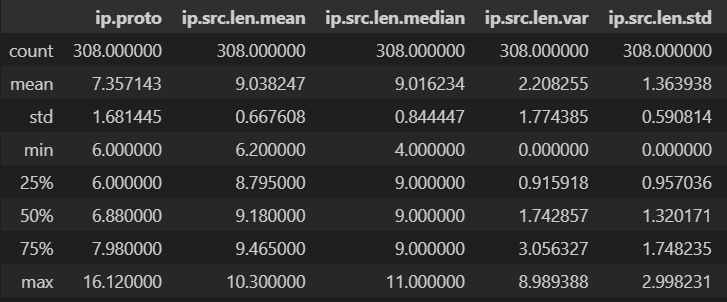
\includegraphics[width=1\textwidth]{./assets/images/describe.png}
	\caption{Describing the dataset}
\end{figure}

\subsection{Distribution of the status column}
 We used \textbf{displot()} from \textbf{seaborn} to plot the distribution of the status column. 0 is the DDoS traffic and 1 is the normal traffic.
\begin{figure}[h]
	\centering
	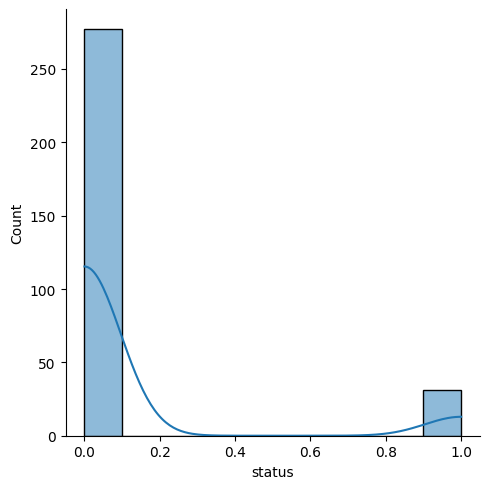
\includegraphics[width=0.8\textwidth]{./assets/images/distribution.png}
	\caption{Distribution of the status column}
\end{figure}

\pagebreak \subsection{Histograms of the variables}
Then we plotted the histograms for each variable :
\begin{figure}[h]
	\centering
	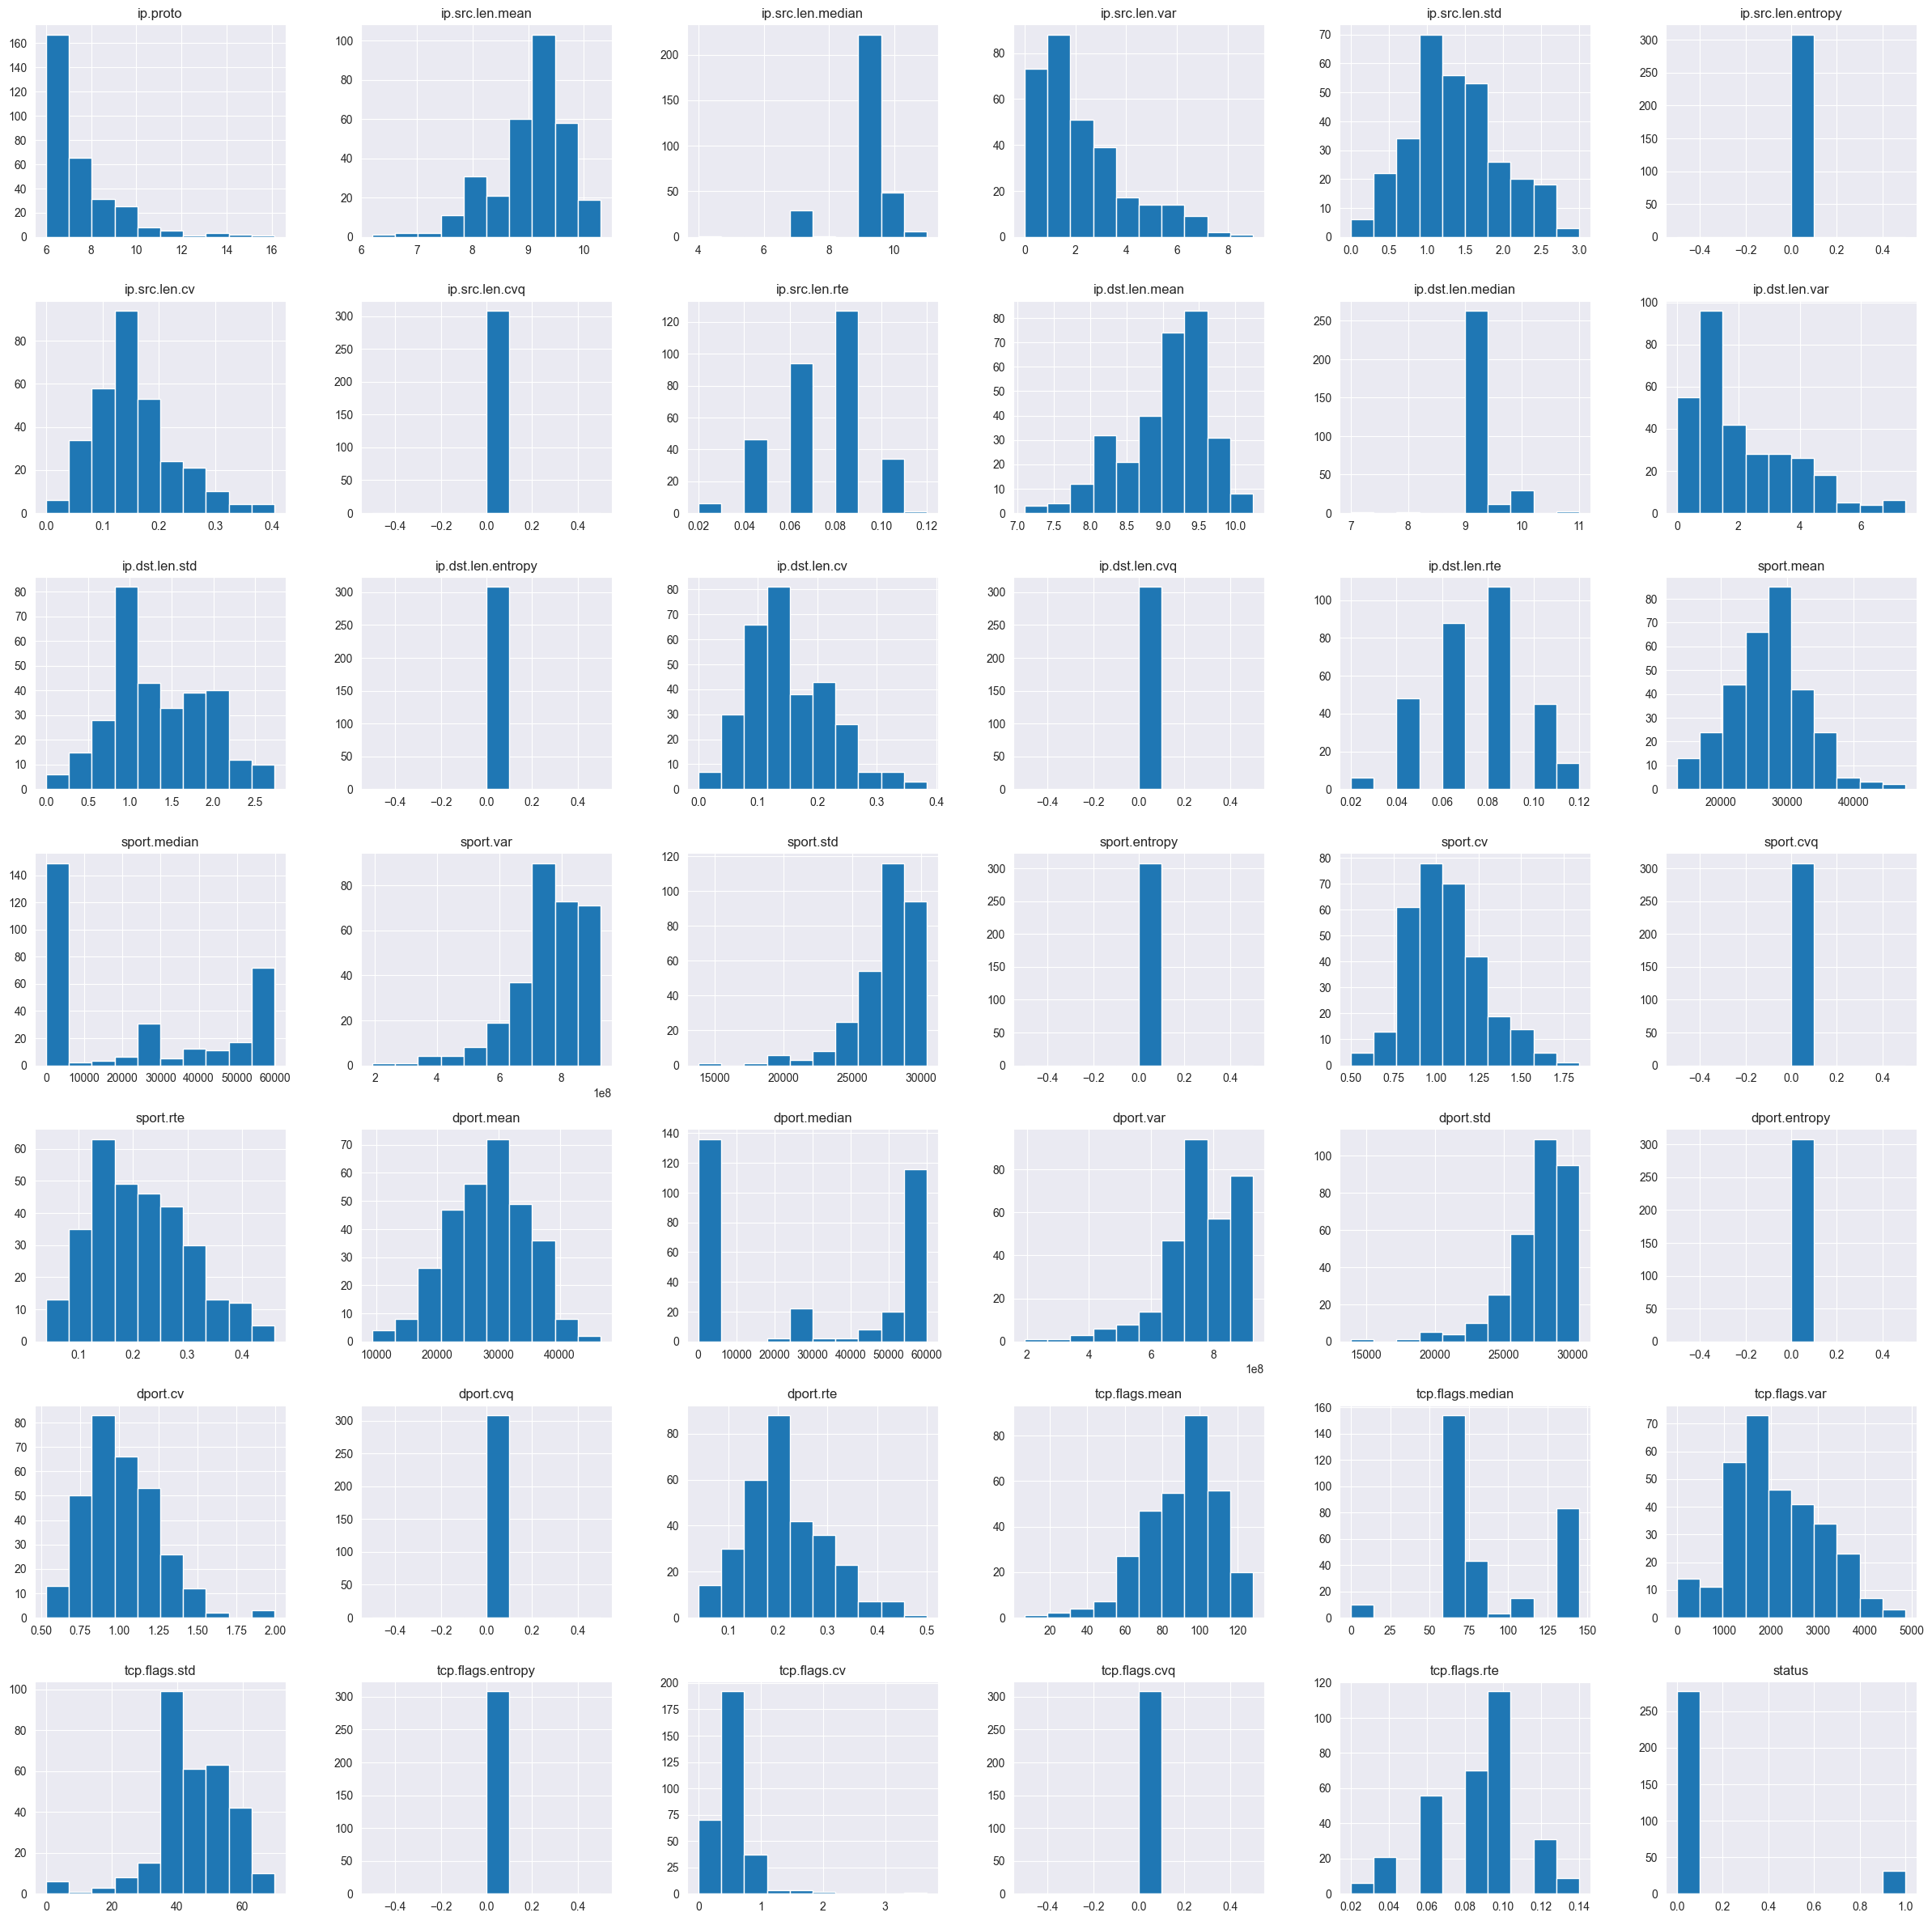
\includegraphics[width=1\textwidth]{./assets/images/hist.png}
	\caption{Histograms of the variables}
\end{figure} 

\subsection{Boxplots}
Boxplots are useful for visually summarizing the distribution of a dataset, identifying outliers and comparing the distribution of the variables. They provide a compact way to display key statistical information about the data.

\subsection{Correlation between different attributes}
\begin{figure}[h]
	\centering
	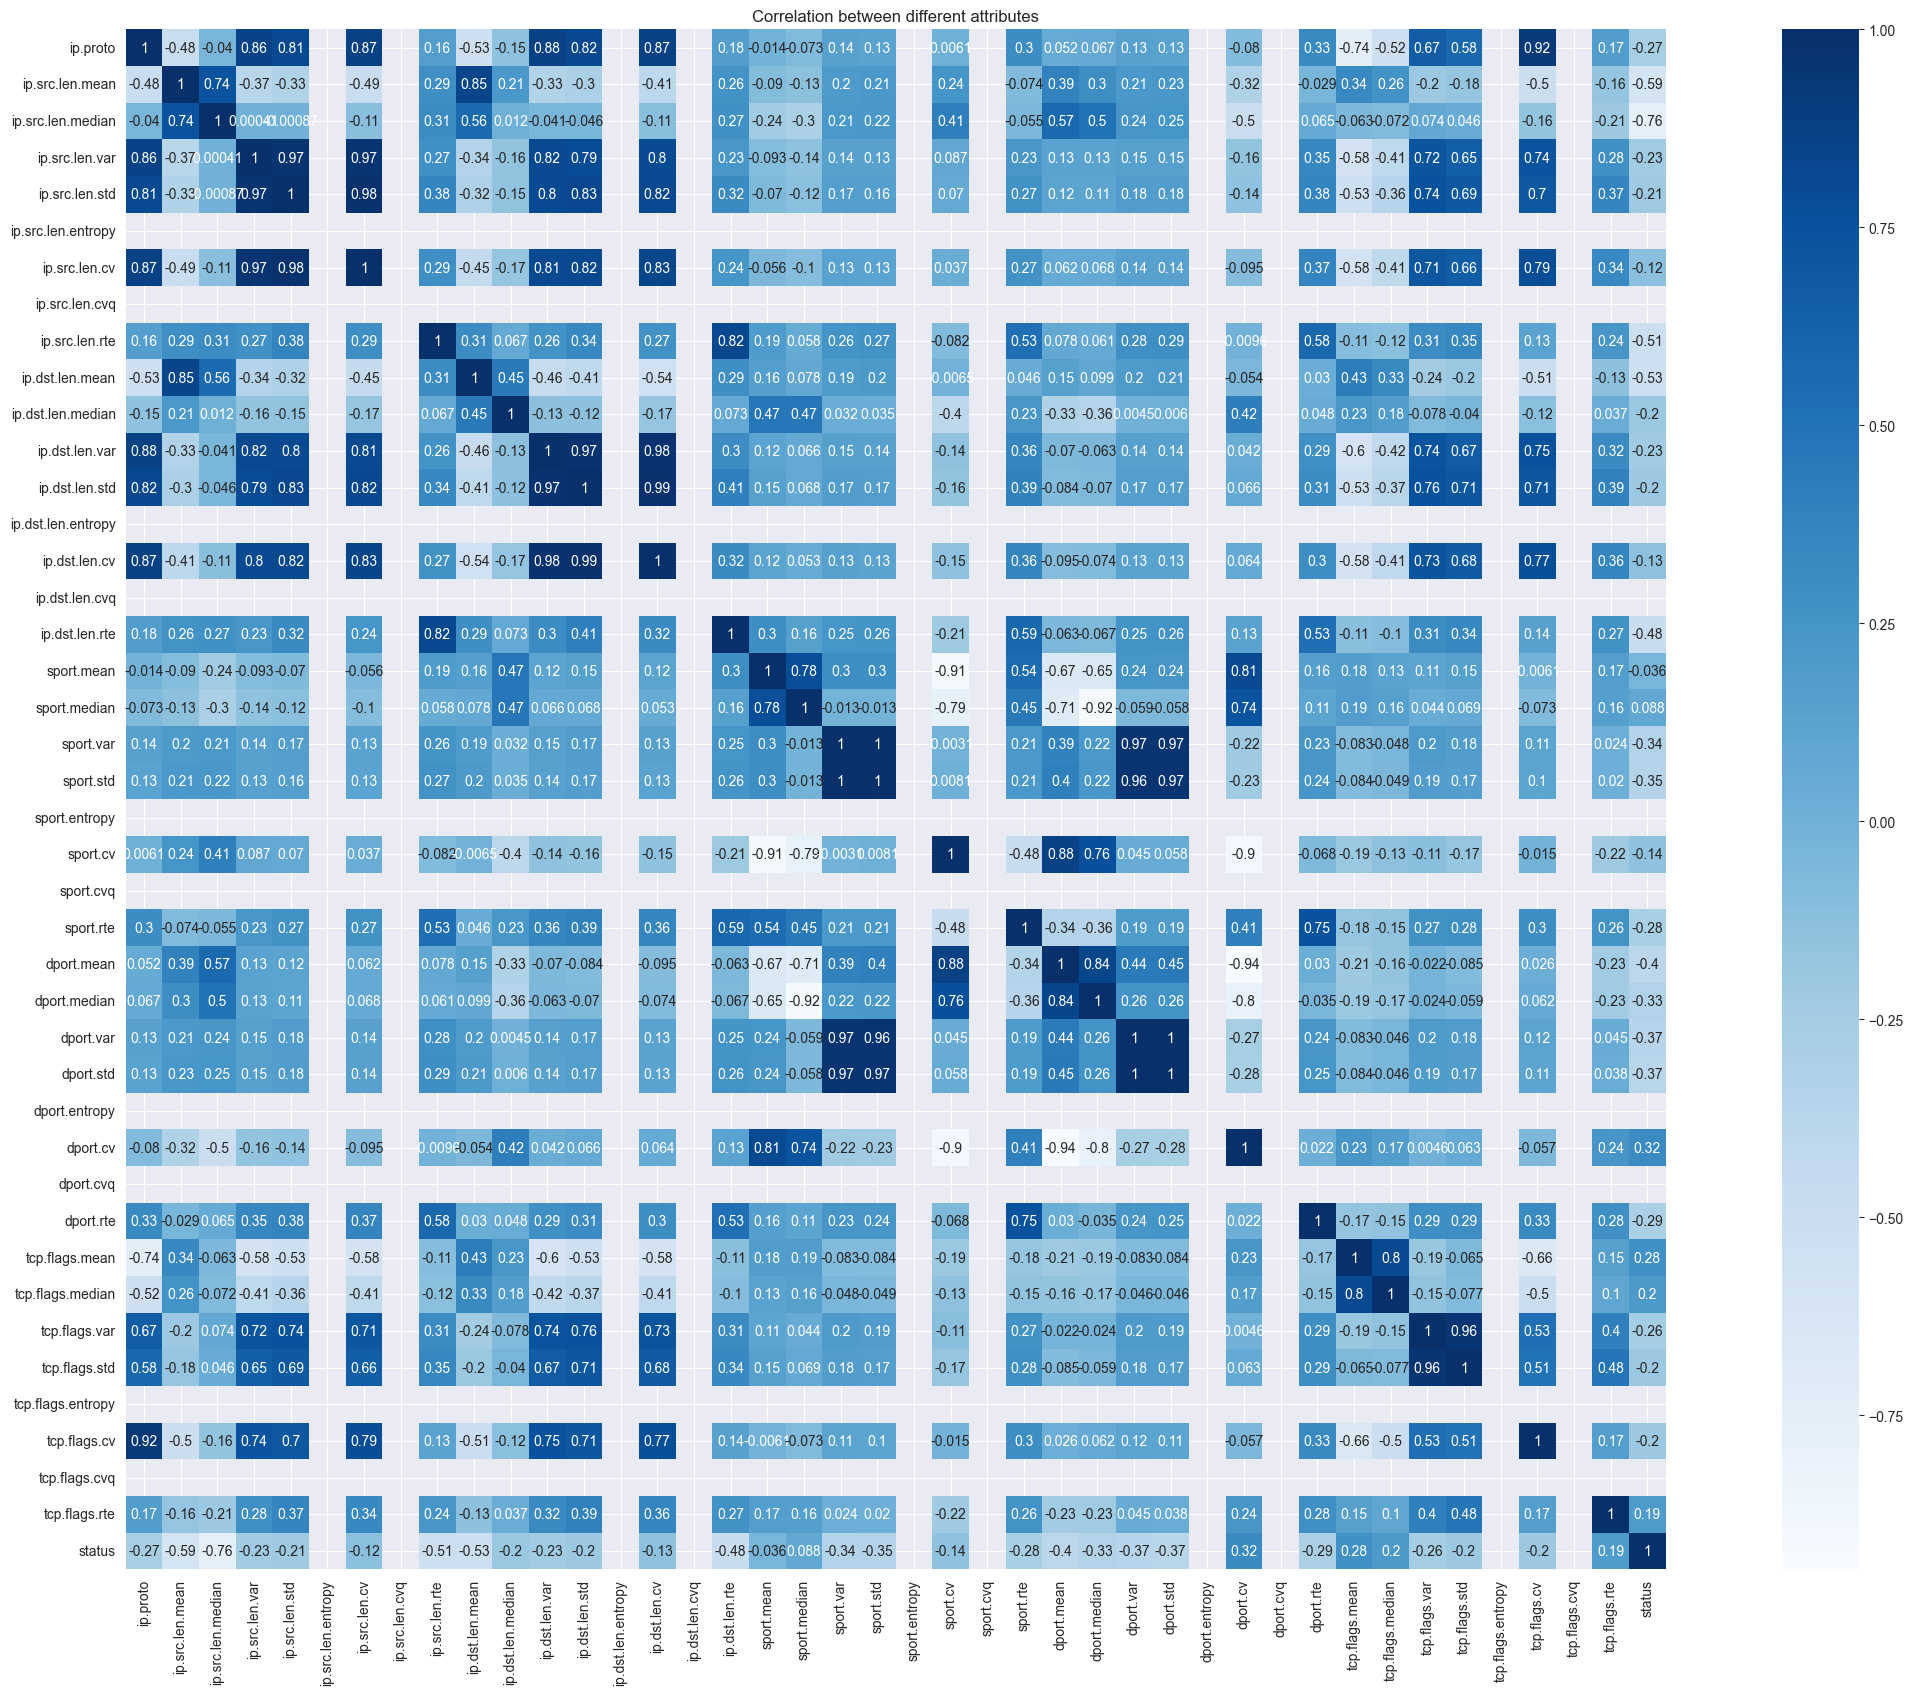
\includegraphics[width=1\textwidth]{./assets/images/correlation.png}
	\caption{Correlation between different attributes}
\end{figure}

